% Instructions to change to html version:
% Comment out:
%  minipage, multicols,columnbreak, mathbf, hrule
% Replace all: \begin{minipage}% \end{minipage} %\begin{multicols}  %\end{multicols} 
% \columnbreak
 %	%% \begin{framed} %\end{framed} %%\hrule
% Replace \mathbf with	\boldsymbol
% Replace $$ with \[ or \]and $ with \( or \)
% Enclose graphics in figure environments and add captions
% 			search \includegraphics
% Re-tag \df environments as sections, subsections, etc.
% Command Line Code to Create html version:
%First: pdflatex -shell-escape filename.tex                                   
%Second, for each figure: inkscape "filename-figure1.pdf" -o "filename-figure1.png"
% Third: htlatex filename.tex "ht5mjlatex.cfg, charset=utf-8" " -cunihtf -utf8"

\documentclass[10pt]{article}

%\usepackage{tikz, pgf,pgfplots,wasysym,array}
%\usepackage{wasysym,array}

\usepackage{amsmath,amssymb}
\usepackage[hidelinks]{hyperref}

\ifdefined\HCode
  \def\pgfsysdriver{pgfsys-tex4ht-updated.def}
\fi 
%\ifdefined\HCode
%  \def\pgfsysdriver{pgfsys-dvisvgm4ht.def}
%\fi 
\usepackage{tikz}
\usetikzlibrary{calc,decorations.markings,arrows}
\usepackage{pgfplots}

\pgfplotsset{compat=1.12}
\usepackage{myexternalize}
\usetikzlibrary{calc,decorations.markings,arrows}
\usepackage{framed}
\usepackage[none]{hyphenat}

\input{../../../common/1336_header_test.tex}
\begin{document}

\newcommand{\an}{\lbrace a_n \rbrace}
\newcommand{\Sum}{\sum_{n=1}^\infty }

\everymath{\displaystyle}

\renewcommand{\myTitle}{MATH 1336: Calculus III}

\renewcommand{\mySubTitle}{Section 5.4, Part 2: Series Tests Practice}
% NOTE: This activity is meant to be used before covering the Alternating Series Test, Absolute/Conditional Convergence, and Ratio/Root Tests.
%~\hfill Name: \underline{~~~~~~~~~~~~~~~~~~~~~~~~~~~~~~~~~~~~~~~~~~~~~~~}

\lectTitle{\vspace*{-.5in}\myTitle}{\vspace*{.1in}\mySubTitle \vspace*{-.25in}}

\section*{Problems for Group Work:}
\textbf{Be sure to fully justify your reasoning as a part of your solutions.}\\
 The answers are upside-down on the bottom of this page.

%\begin{framed}
For Problems \ref{prob1}-\ref{prob5}, determine whether the series is convergent, divergent, or if we cannot determine the convergence behavior using the tests we know at this point.
%\emnd{framed}

\begin{enumerate}

%\begin{multicols}{2}

\item \(\Sum \frac{1}{n^2+1}\) \label{prob1}
%Converge
\vspace*{.5in}

\item \(\Sum \frac{n}{n^2+1}\) \label{prob2}
%Diverge
\vspace*{.5in}

\item \(\Sum \frac{\cos(n)\sqrt{n}}{3n+4}\) \label{prob3}
%Cannot Determine
\vspace*{.5in}

\item \(\Sum \int_{n}^{n+1} \frac{dx}{x^{2/3}}\) \label{prob4}
%Diverge
\vspace*{.5in}

\item \(\Sum 2^{-n} a_n\), where \(a_n = f(n)\) as shown below: \label{prob5}
%Converge

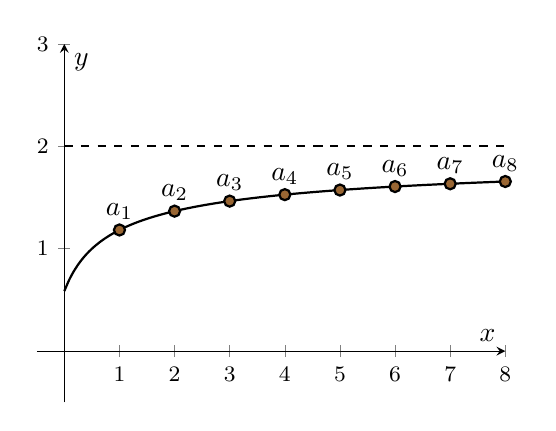
\begin{tikzpicture}
\begin{axis}[
	y=1.3cm,
    x=0.7cm,
	axis x line=middle,
	axis y line = middle,
	ymin=-.5,ymax=3,
	xmin=-.5,xmax=8,
    grid=none,
    xtick={-0,...,8},
    ytick={-0,...,3},
    xlabel=\(x\),
    ylabel=\(y\),
    tick label style={font=\footnotesize}
]
%\addplot[domain=0:1.9,mark=none, thick] {1-x};
%%\addplot[domain=0:1,mark=none, thick] {1};
%\addplot[domain=-2:0,mark=none, thick] {sqrt(1-(x+1)^2)+1};

\addplot[domain=0:8,mark=none, thick, smooth, samples=100]{-1/(x+.5)^.5+2};
\addplot[domain=0:8,mark=none, thick, dashed]{2};
\addplot+[domain=1:8,only marks, mark=*,  thick , black, samples=8, nodes near coords={\(a_{\pgfmathprintnumber[fixed,precision=1]{\pgfkeysvalueof{/data point/x}}}\)}] {-1/(x+.5)^.5+2};
%\addplot+[only marks, mark=o,  thick , black] coordinates {(2,6)};



%\node  at (axis cs:  5, 5) {\(g\)};

\end{axis}
\end{tikzpicture}

\vspace*{.5in}
%\end{multicols}

%\begin{framed}
%For Problem \ref{prob6}, determine whether the series is convergent or divergent by expressing \(s_n\) as a telescoping sum. If it is convergent, find its sum.
%\end{framed}
%\item \(\sum_{n=2}^\infty \frac{2}{n^2-1}\) \label{prob6}
%%Converges to \(\frac{3}{2}\).
%%\vfill


\end{enumerate}

\vfill

\rotatebox{180}{
%\begin{minipage}{\textwidth}
\underline{Answers:}\\\textbf{Problem \ref{prob1}:} Converge, 
\textbf{Problem \ref{prob2}:} Diverge, 
\textbf{Problem \ref{prob3}:} Cannot Determine, 
\textbf{Problem \ref{prob4}:} Diverge,\\
\textbf{Problem \ref{prob5}:} Converge,
%\textbf{Problem \ref{prob6}:} Converges to \(\tfrac{3}{2}\)
%\end{minipage}
}

\end{document}
